\documentclass{beamer}
\usetheme{metropolis}

\usepackage[ngerman]{babel}
\usepackage[autostyle=true,german=quotes]{csquotes}
\usepackage[linewidth=1pt]{mdframed}
\usepackage{hyperref}
\usepackage{makecell}
\usepackage{pifont}
\usepackage{tikz}
\usetikzlibrary{positioning, calc, arrows, fit, decorations.pathreplacing, shapes, shapes.multipart, snakes}
\usepackage{verbatim}
\usepackage{tabularx}
\usepackage{textcomp}
\usepackage{centernot}
\usepackage{amsmath}
\usepackage{xcolor}
\usepackage{tikz}
\usepackage{underscore}
%\usepackage{pdfpages}

\batchmode

\hypersetup{
	colorlinks,
	urlcolor=blue,
	linkcolor=black % for ToC
}
\newenvironment{qaa}[1]{
	#1

	\begin{mdframed}
		\small
}{
	\end{mdframed}
}

\newcommand{\true}{\ding{51}}
\newcommand{\false}{\ding{55}}
\newcommand{\code}[1]{
	\begin{mdframed}
		\verbatiminput{#1}
	\end{mdframed}
}

\title{Tutorium 09: Parallelität in Java}
% \subtitle{}
\author{Paul Brinkmeier}
\institute{Tutorium Programmierparadigmen am KIT}
\date{19. Januar 2020}

\begin{document}

\begin{frame}
	\titlepage
\end{frame}

\section{Heutiges Programm}

\begin{frame}{Parallelprogrammierung}
	ProPa-Stoff zu Parallelprogrammierung:

	\begin{itemize}
		\item Grundlegende Begriffe
		\item Message Passing, wurde in OS \emph{kurz} behandelt (\enquote{message queues})
		\item Shared Memory + Synchronisierung, wie in SWT1, OS, etc.
		\begin{itemize}
                  \item In Java, mit ein paar Details zur JVM \textcolor{red}{$\leftarrow$ wir sind hier}
		\end{itemize}
              \item Dieses Jahr: \emph{Manuelles Threading und Monitore in Java (siehe bspw. auch SWT1) sind nicht Bestandteil der VL.}
	\end{itemize}
\end{frame}

\begin{frame}{Parallelprogrammierung}
  Heute: Verschiedene Java-/Parallelprogrammierungskonzepte

  \begin{itemize}
    \item Amdahlsches Gesetz
    \item Lambdas, \texttt{@FunctionalInterface}
    \item Threads (\texttt{.start()}, \texttt{.run()})
    \item Happens-before-Beziehung
  \end{itemize}
\end{frame}

\section{Wiederholung}

\begin{frame}{Flynns Taxonomie}
	\begin{itemize}
		\item SISD: Single Instruction, Single Data\\
			{\footnotesize Ein Datum wird von einer Ausführungsarbeit bearbeitet}
		\item SIMD: Single Instruction, Multiple Data\\
			{\footnotesize Eine Ausführungseinheit bearbeitet mehrere Daten gleichzeitig}
		\item MIMD: Multiple Instruction, Multiple Data\\
			{\footnotesize $\approx$ Mehrere Ausführungseinheiten arbeiten gleichzeitig}
		\item MISD: Multiple Instruction, Single Data\\
			{\footnotesize $\approx$ Mehrere Ausführungseinheiten arbeiten gleichzeitig an einem Datum}
	\end{itemize}
\end{frame}

\begin{frame}{Daten- und Taskparallelismus}
	Parallele Probleme sind üblicherweise entweder
	
	\begin{itemize}
		\item \enquote{datenparallel}: Problem kann auf identische Ausführungseinheiten verteilt werden\\
			Beispiel: \texttt{map primeFactors [1432793, 651433, ...]}

		\item \enquote{taskparallel}: Problembestandteile sind nicht homogen\\
			Beispiel: Videospiel mit Render-, Netzwerk- und Logikprozessen
	\end{itemize}

	Datenparallele Probleme sind i.d.R. einfacher zu behandeln (auch: \enquote{embarrassingly parallel}).
	Bei manchen Problemen verschwimmt die Grenze auch (bspw. Webserver).
\end{frame}

\begin{frame}{MPI}
	MPI (\enquote{Message Passing Interface}) ist ein Standard für Parallelprogrammierung.
	Es existieren verschiedene Implementierungen für verschiedene Sprachen.
	Die VL verwendet \href{https://www.open-mpi.org/}{Open MPI}, eine Open-Source-Implementierung.

	\begin{itemize}
		\item MPI-\enquote{Prozesse} beziehen sich i.d.R. auf Prozessorkerne
		\item Message Passing statt Shared Memory:
		\begin{itemize}
			\item Daten werden explizit über \texttt{Send} und \texttt{Recv} geteilt
		\end{itemize}
		\item MPI-Prozesse werden in sog. \emph{Communicators} eingeteilt. Wir verwenden immer den Communicator, der alle Prozesse enthält (\texttt{MPI_COMM_WORLD)})
	\end{itemize}
\end{frame}

\newcolumntype{C}{p{0.4cm}}

\begin{frame}{MPI: Kollektive Operationen}
        Statt \texttt{Send} und \texttt{Recv} nutzt man in MPI meistens \enquote{kollektive Operationen}.

        \begin{itemize}
          \item \emph{Selber Aufruf in jedem Prozess}
          \item Meistens mit \texttt{root} Parameter, um Datenquelle zu bestimmen
        \end{itemize}

        Beispiel: \texttt{Bcast} verteilt ein Datum auf alle Prozesse.

	\begin{figure}
	\begin{tikzpicture}
		\node (lhs) {\begin{tabular}{|C|C|C|}
			\hline
			$A_0$ & & \\
			\hline
			& & \\
			\hline
			& & \\
			\hline
		\end{tabular}};
		\node (lhsLabelP) [left=0 of lhs] {\rotatebox{90}{\tiny Prozesse}};
		\node (lhsLabelD) [above=0 of lhs] {\tiny Daten};

		\node (rhs) [right=4cm of lhs] {\begin{tabular}{|C|C|C|}
			\hline
			$A_0$ & & \\
			\hline
			\textcolor{blue}{$A_0$} & & \\
			\hline
			\textcolor{blue}{$A_0$} & & \\
			\hline
		\end{tabular}};

		\draw[->, thick] (lhs) -- node[above] {\texttt{Bcast(root=0)}} (rhs);
	\end{tikzpicture}
	\end{figure}
\end{frame}

\begin{frame}{Cheatsheet: Liste an kollektiven MPI-Operationen}
  Folgende kollektiven Operationen kennen wir:

  \begin{itemize}
    \item \texttt{MPI_Bcast}
    \item \texttt{MPI_Scatter}, \texttt{MPI_Gather}
    \item \texttt{MPI_Allgather} (\enquote{\texttt{Gather}} + \texttt{Bcast})
    \item \texttt{MPI_Alltoall} (\enquote{transponiert})
    \item \texttt{MPI_Reduce} (\enquote{wie \texttt{fold}})
  \end{itemize}

	\begin{figure}
	\begin{tikzpicture}
		\node (lhs) {\begin{tabular}{|C|C|C|}
			\hline
			$A_0$ & $A_1$ & $A_2$ \\
			\hline
			$B_0$ & $B_1$ & $B_2$ \\
			\hline
			$C_0$ & $C_1$ & $C_2$ \\
			\hline
		\end{tabular}};
		\node (lhsLabelP) [left=0 of lhs] {\rotatebox{90}{\tiny Prozesse}};
		\node (lhsLabelD) [above=0 of lhs] {\tiny Daten};

		\node (rhs) [right=4cm of lhs] {\begin{tabular}{|C|C|C|}
			\hline
			\textcolor{blue}{$A_0$} & \textcolor{blue}{$B_0$} & \textcolor{blue}{$C_0$} \\
			\hline
			\textcolor{blue}{$A_1$} & \textcolor{blue}{$B_1$} & \textcolor{blue}{$C_1$} \\
			\hline
			\textcolor{blue}{$A_2$} & \textcolor{blue}{$B_2$} & \textcolor{blue}{$C_2$} \\
			\hline
		\end{tabular}};

		\draw[->, thick] (lhs) -- node[above] {\texttt{Alltoall()}} (rhs);
	\end{tikzpicture}
	\end{figure}
\end{frame}

\section{Amdahlsches Gesetz}

\begin{frame}{Amdahlsches Gesetz}
  Gegeben den parallelisierbaren Anteil eines Algorithmus $p \in [0, 1]$, berechnet

  \begin{equation*}
    S(n) = \frac{T(1)}{T(n)} = \frac{1}{(1 - p) + \frac{p}{n}}
  \end{equation*}

  den \emph{maximalen Speedup} durch parallele Ausführung auf $n$ Prozessoren.

  \only<1>{
  \begin{itemize}
    \item \emph{In der Praxis nicht erreichbar durch OS-Overhead!}
    \item Trotzdem gute Annäherung für die etwaige Größenordnung des tatsächlichen Speedups (wenn man $p$ kennt)
  \end{itemize}
  }

  \only<2>{
  Beispielalgorithmus (Histogramm eines Graustufenbildes berechnen):
  \begin{itemize}
    \item Berechne Histogramme für Bildauschnitte (7s, parallelisierbar)
    \item Summiere einzelne Histogramme (3s, nicht parallelisierbar)
  \end{itemize}
  }

  \only<3>{
    \begin{align*}
      P &= \frac{7s}{7s + 3s} = 0,7 \\
      T(n) &= 0.3 + \frac{0,7}{n} \\
      S(4) &= \frac{1}{0,3 + 0,175} \approx 2,1
    \end{align*}
  }
\end{frame}

\section{\texttt{@FunctionalInterface}}

\begin{frame}{Lambdas}
  Seit Java 8 gibt es Lambda-Ausdrücke, bspw.:

  \code{code/funcinterface.java}

  Ein Lambda ist hier Syntaxzucker für eine anonyme Klassendeklaration (gabs auch schon vor Java 8):

  \code{code/anonymousclass.java}
\end{frame}

\begin{frame}{Das Interface \texttt{Function}}
  \code{code/function.java}

  \begin{itemize}
    \item \text{java.util.function} enthält alle möglichen solchen Interfaces (ziemlicher Clusterfuck)
    \item Eigene Typen für Lambdas?
  \end{itemize}
\end{frame}

\begin{frame}{\texttt{@FunctionalInterface}}
  Um eigene Typen für Lambdas zu definieren, können wir Interfaces mit einer einzelnen Methode schreiben und diese als \texttt{@FunctionalInterface} annotieren:

  \code{code/myfuncinterface.java}

  Das können wir verwenden, um nicht überall \texttt{Function<A, B>} stehen zu haben.
\end{frame}

\section{Threads in Java}

\begin{frame}{Manuelle Threadverwaltung in Java}
  \code{code/runnable.java}

  \begin{itemize}
    \item Functional interfaces können für ad-hoc Threads verwendet werden
    \item Threadverwaltung:
    \begin{itemize}
      \item \texttt{t.start()} lässt den Thread \texttt{t} anlaufen
      \item \texttt{t.join()} wartet bis \texttt{t} durchgelaufen ist
      \item Außerdem: \texttt{interrupt()}/\texttt{isInterrupted()}
    \end{itemize}
  \end{itemize}
\end{frame}

\begin{frame}{Aufgabe: Thread-Programmierung}
  Parallelisiert ein Programm, das das Graustufenhistogramm eines Bildes berechnet.

  \only<1>{
  \begin{figure}
    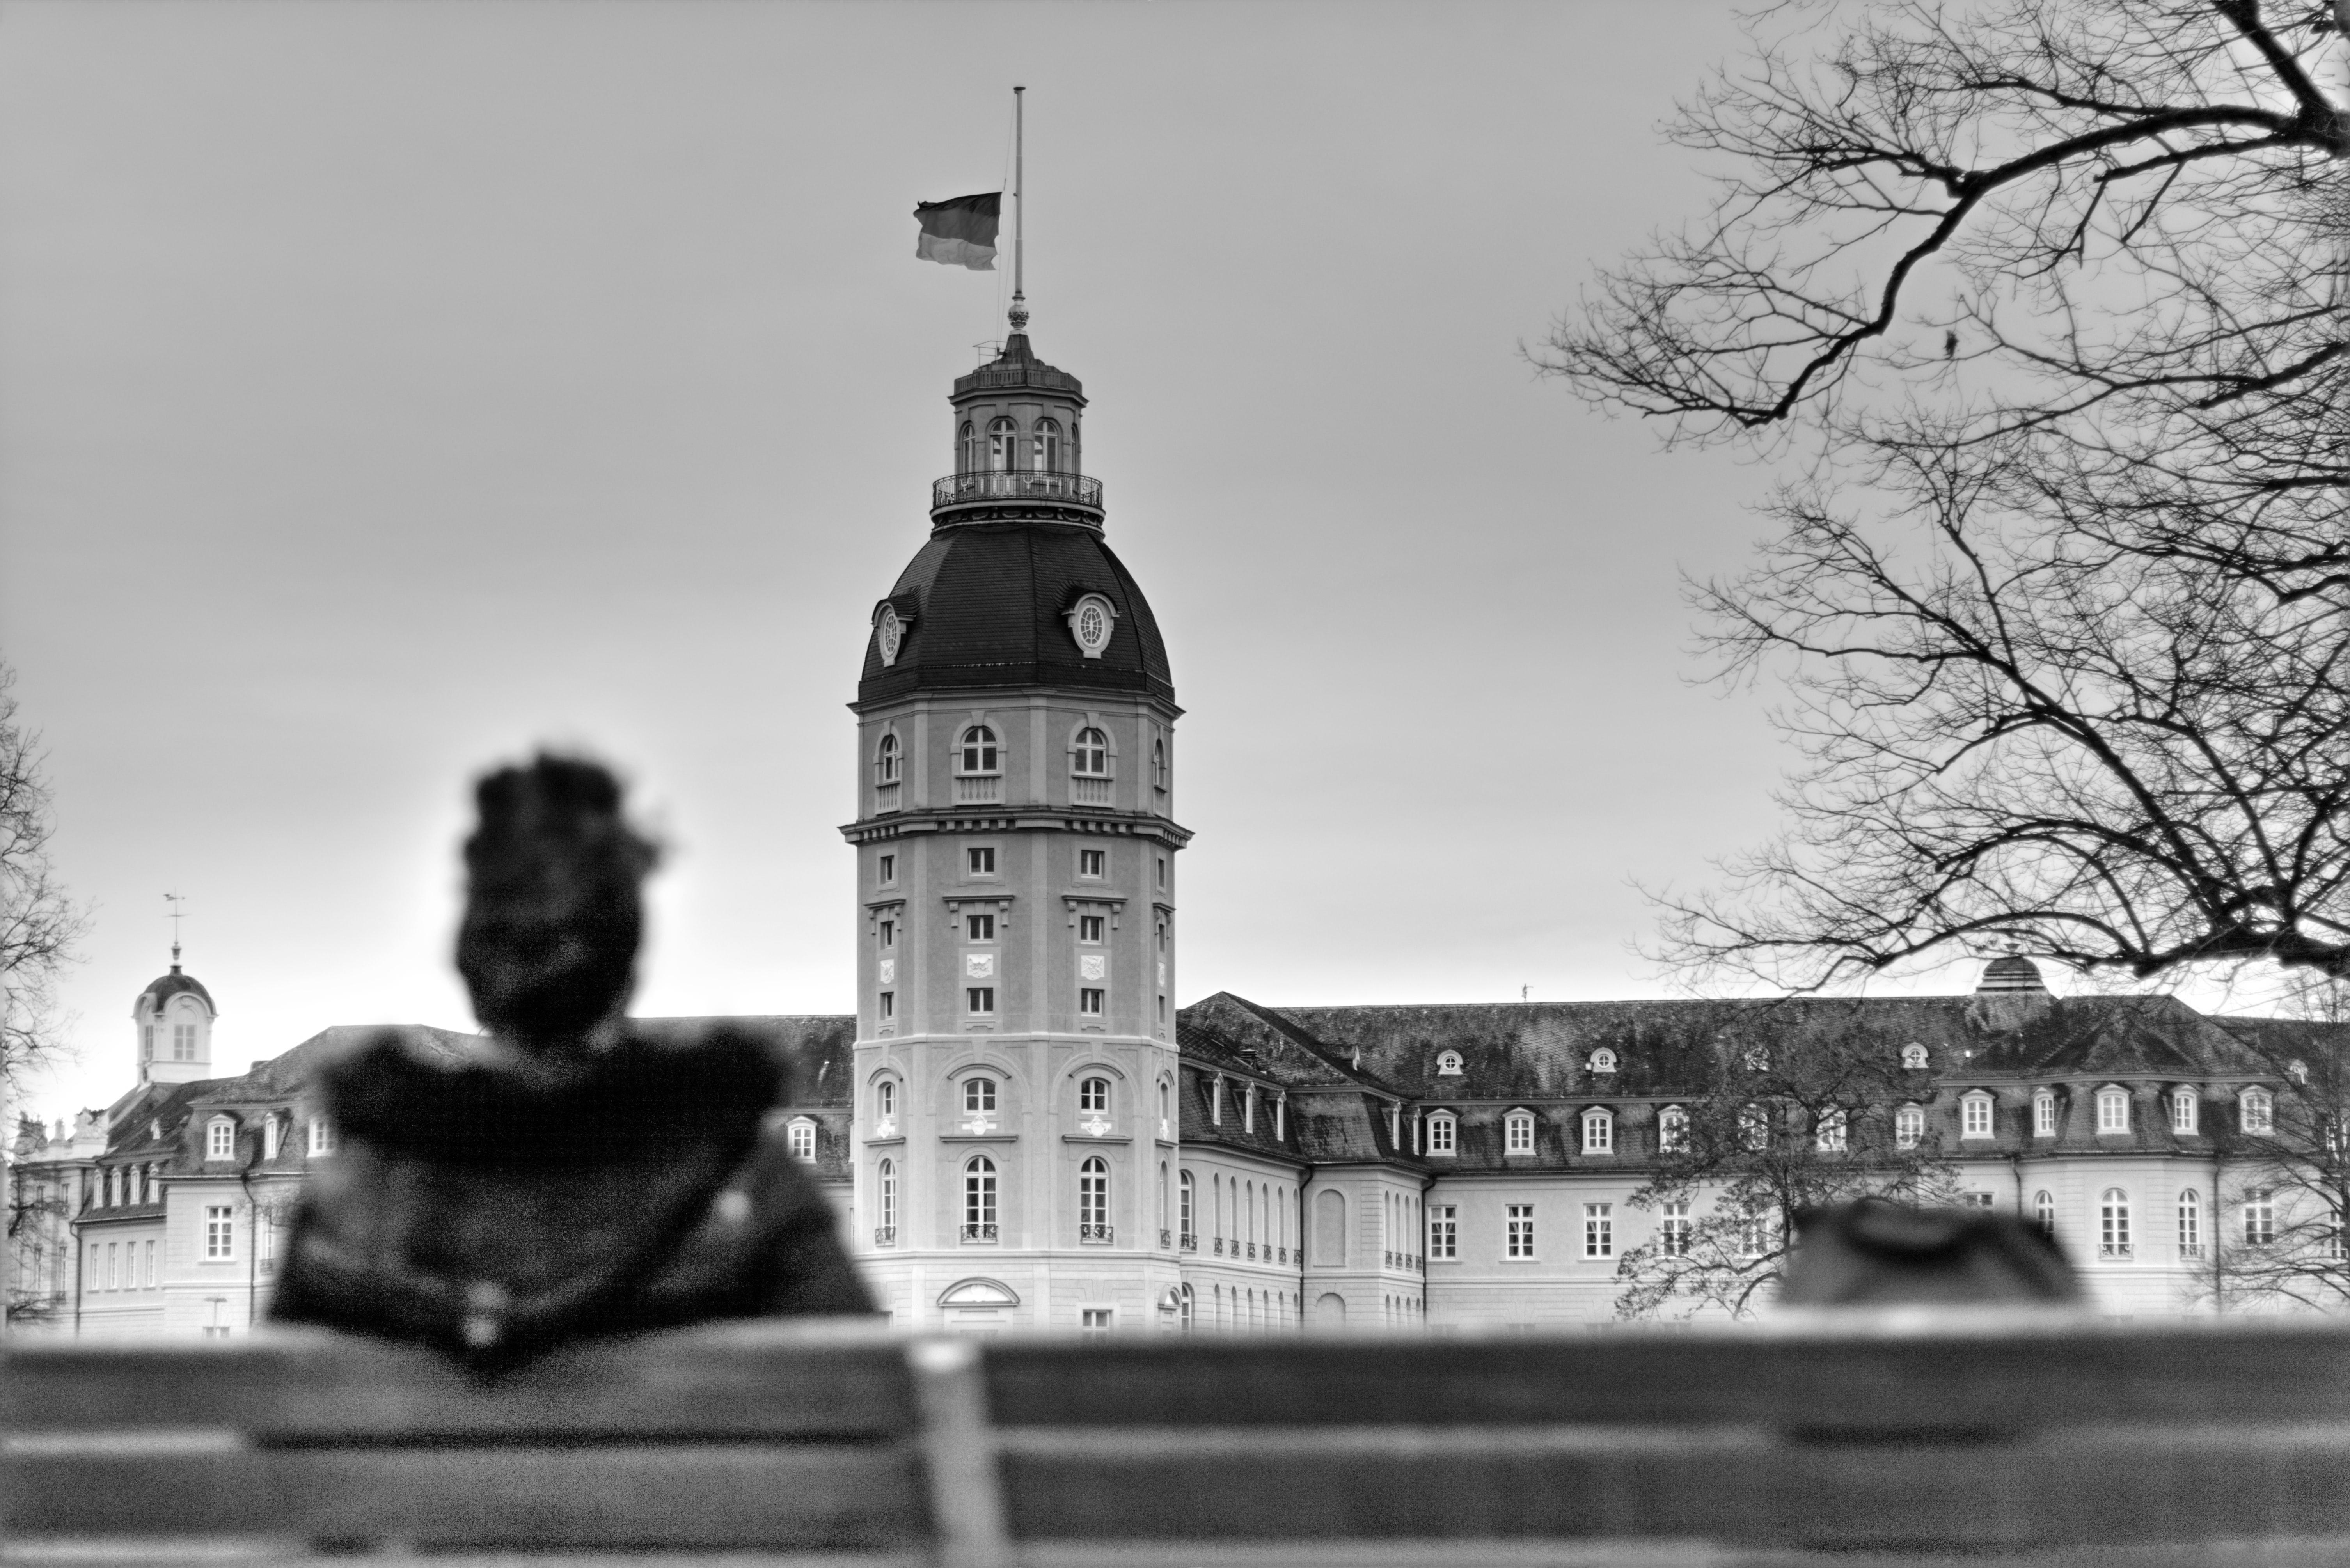
\includegraphics[width=0.7\textwidth]{images/schloss.gray.jpg}
  \end{figure}
  }

  \only<2>{
    \begin{itemize}
      \item Programm lädt Graustufenbild als Array von Bytes (0 = schwarz, 255 = weiß)
      \item Histogramm: Wie oft kommen alle Grauwerte als Pixel vor?
      \item Parallelisiert den Code in \texttt{demos/java/Histogram.java}!
      \begin{itemize}
        \item Verwendet \texttt{Thread}, \texttt{start()} und \texttt{join()}
        \item Vergleicht die resultierende Zeit mit der nicht parallelisierten Version.
        \item Wieviele Kerne hat euer Rechner? Lohnt es sich, mehr Threads zu starten als Kerne verfügbar sind?
      \end{itemize}
    \end{itemize}
  }
\end{frame}

\begin{frame}{Aufgabe: Thread-Programmierung}
  Parallelisiert ein Programm, das das Graustufenhistogramm eines Bildes berechnet.

  \only<1>{
  \begin{figure}
    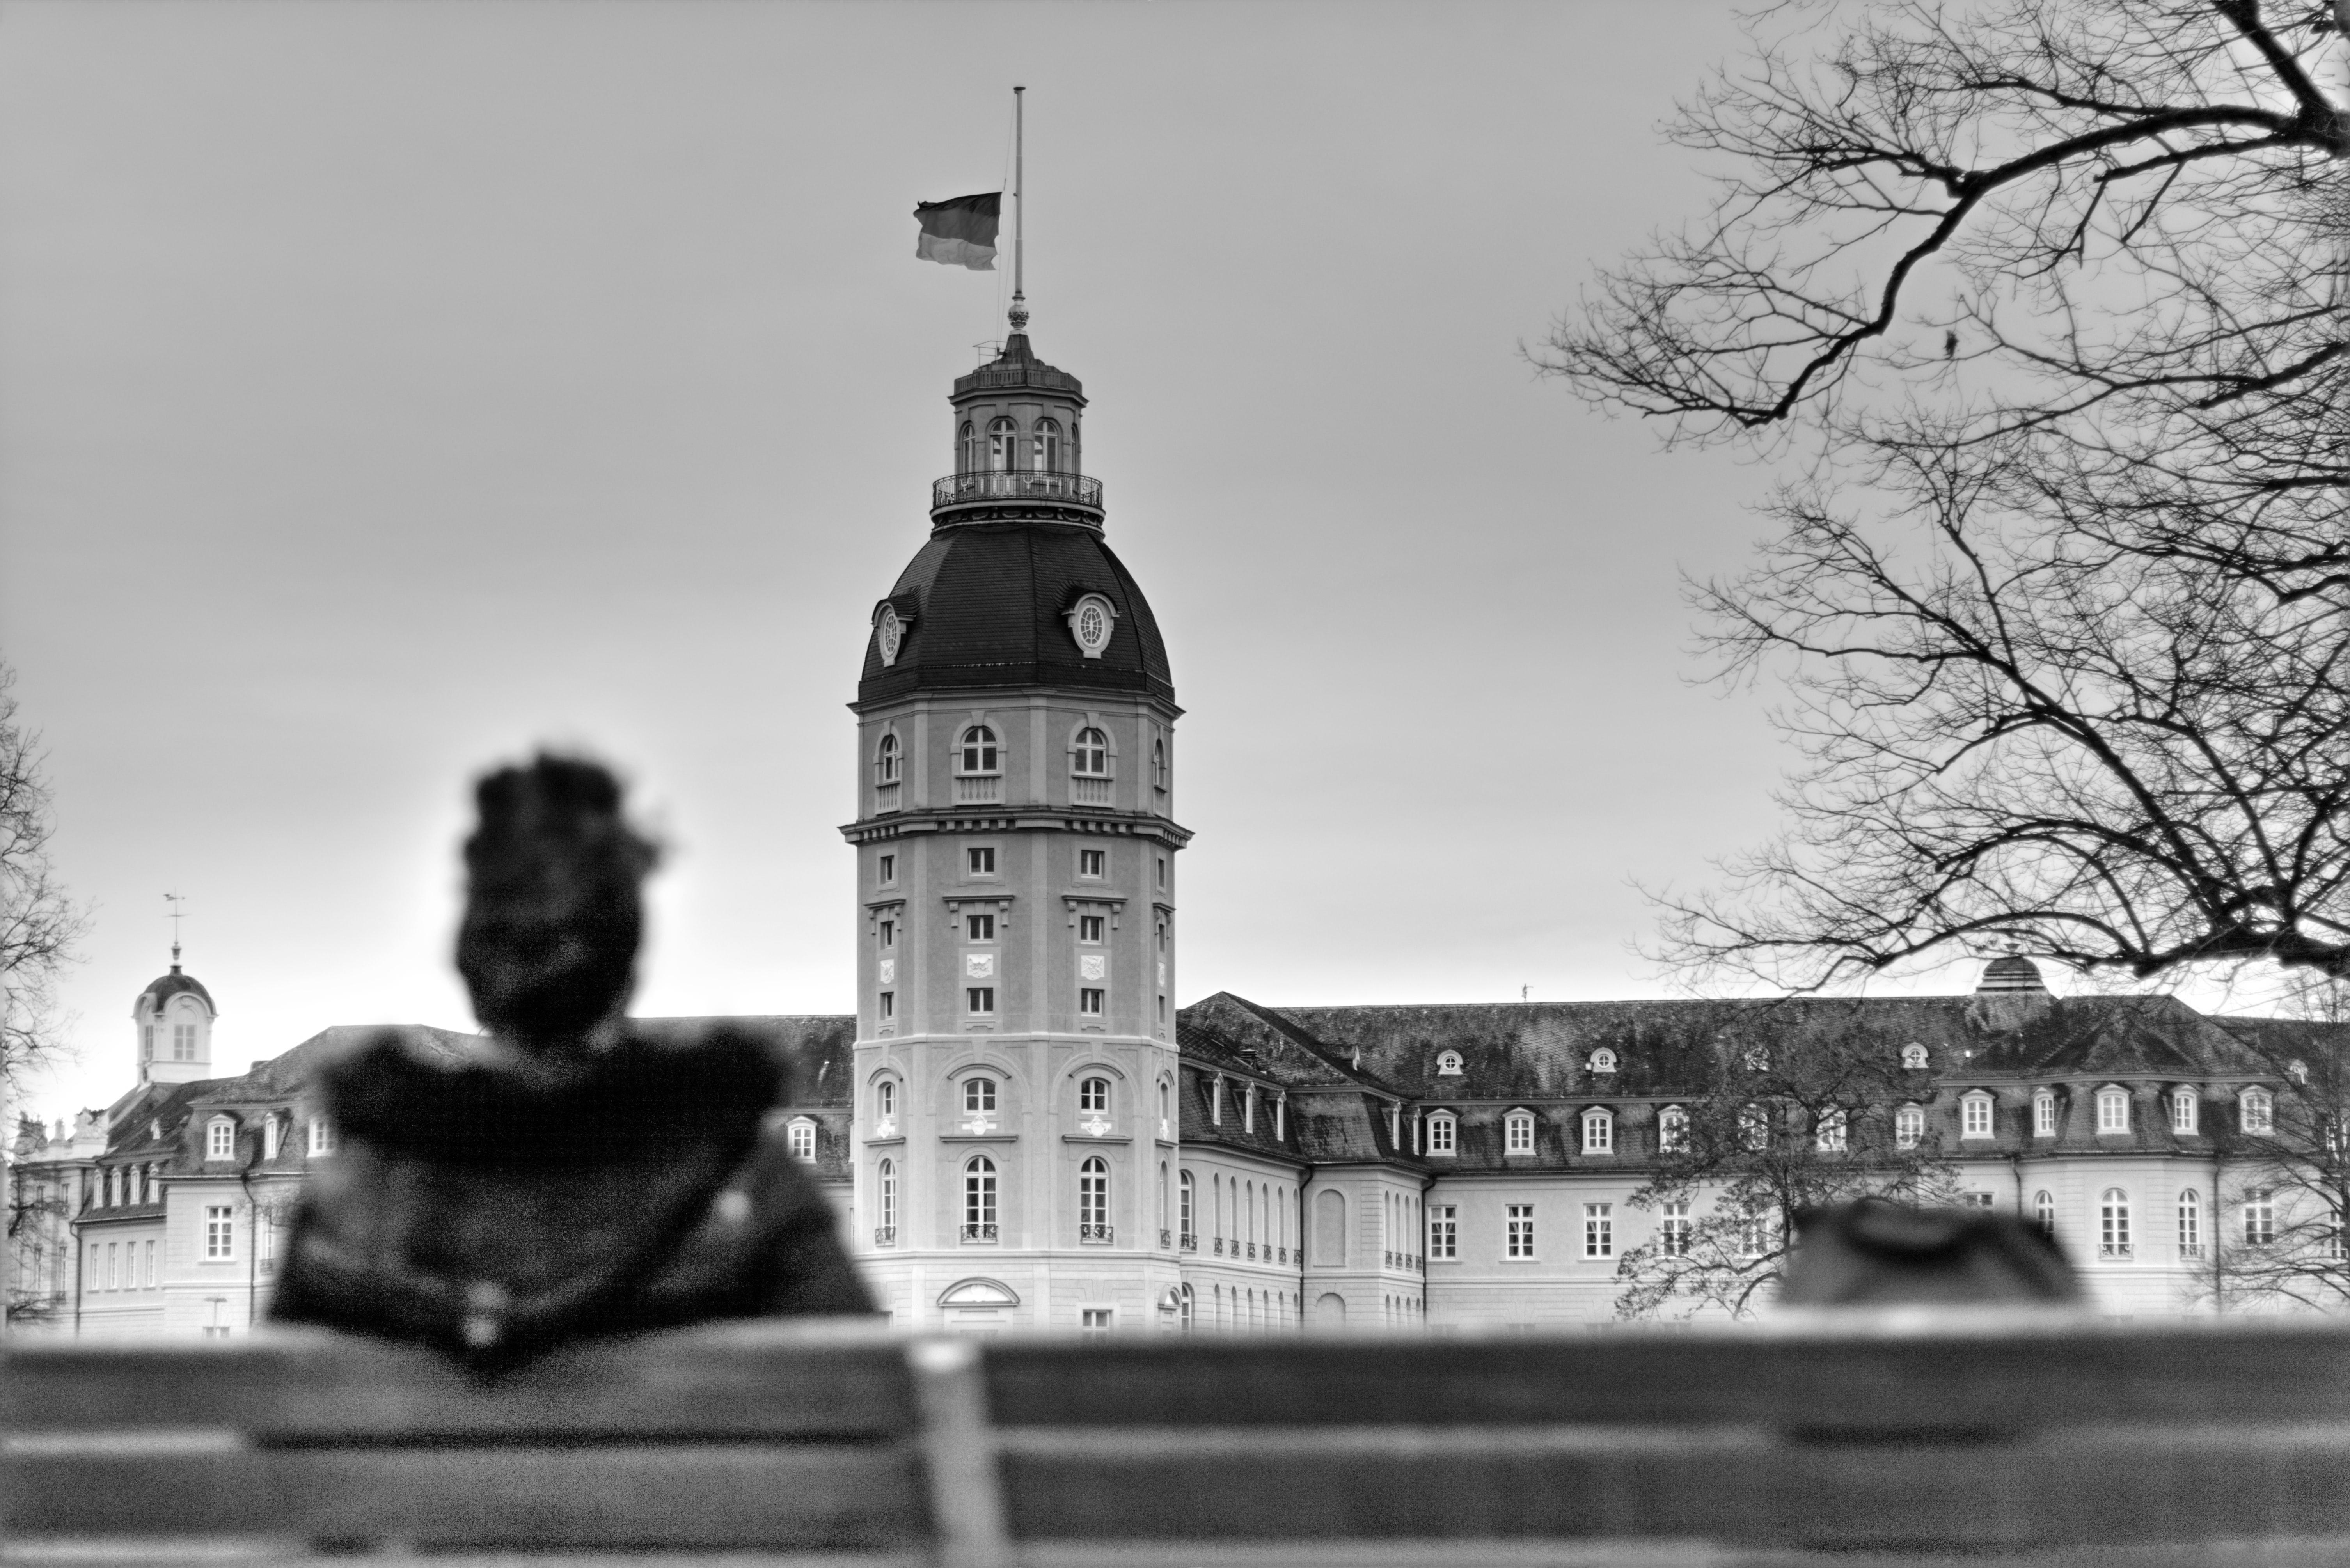
\includegraphics[width=0.7\textwidth]{images/schloss.gray.jpg}
  \end{figure}
  }

  \only<2>{
    \begin{itemize}
      \item Programm lädt Graustufenbild als Array von Bytes (0 = schwarz, 255 = weiß)
      \item Histogramm: Wie oft kommen alle Grauwerte als Pixel vor?
      \item Parallelisiert den Code in \texttt{demos/java/Histogram.java}!
      \begin{itemize}
        \item Verwendet \texttt{Thread}, \texttt{start()} und \texttt{join()}
        \item Vergleicht die resultierende Zeit mit der nicht parallelisierten Version.
        \item Wieviele Kerne hat euer Rechner? Lohnt es sich, mehr Threads zu starten als Kerne verfügbar sind?
      \end{itemize}
    \end{itemize}
  }
\end{frame}

\section{Happens-before}

\begin{frame}{Happens-before-Beziehung}
  \begin{itemize}
    \item TBD
  \end{itemize}
\end{frame}

\section{Ende}

\begin{frame}{Ende}
  % TODO
	\begin{itemize}
		\item Im Campus-System könnt ihr euch bis zum 23.03. für die PP-Klausur anmelden
                \begin{itemize}
                  \item Termin: 09.04.2020 um 17:00, Zelt auf dem Forum :(
                \end{itemize}
		\item \href{https://campus.studium.kit.edu/renewal/payment.php}{Rückmelden} ist möglich bis zum 15.02.
	\end{itemize}
\end{frame}

\end{document}
